
\documentclass[12pt]{article}
\usepackage[margin=1in]{geometry}% Change the margins here if you wish.
\setlength{\parindent}{0pt} % This is the set the indent length for new paragraphs, change if you want.
\setlength{\parskip}{5pt} % This sets the distance between paragraphs, which will be used anytime you have a blank line in your LaTeX code.
\pagenumbering{gobble}% This means the page will not be numbered. You can comment it out if you like page numbers.

\usepackage{amsmath,amsthm,amssymb}

\usepackage{graphicx}
\usepackage{float}
\usepackage{hyperref}
%\usepackage{biblatex}
%\bibliographystyle{}
%\bibliography{syl_references.bib}


\title{Progreso del Chatbot}

\date{}

\begin{document}

\maketitle

\begin{figure}[h]
\caption{Progreso acumulado}
\centering
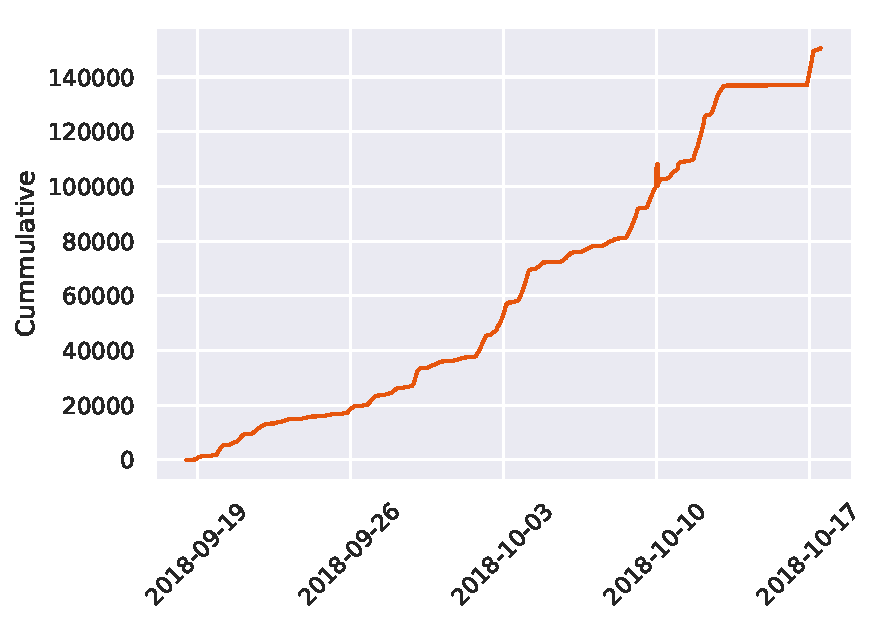
\includegraphics[width=0.75\textwidth]{Cummulative_progress.pdf}
\floatfoot{Insert note here.}
\end{figure}

\begin{figure}[h]
\caption{Frecuencia de interacciones}
\centering
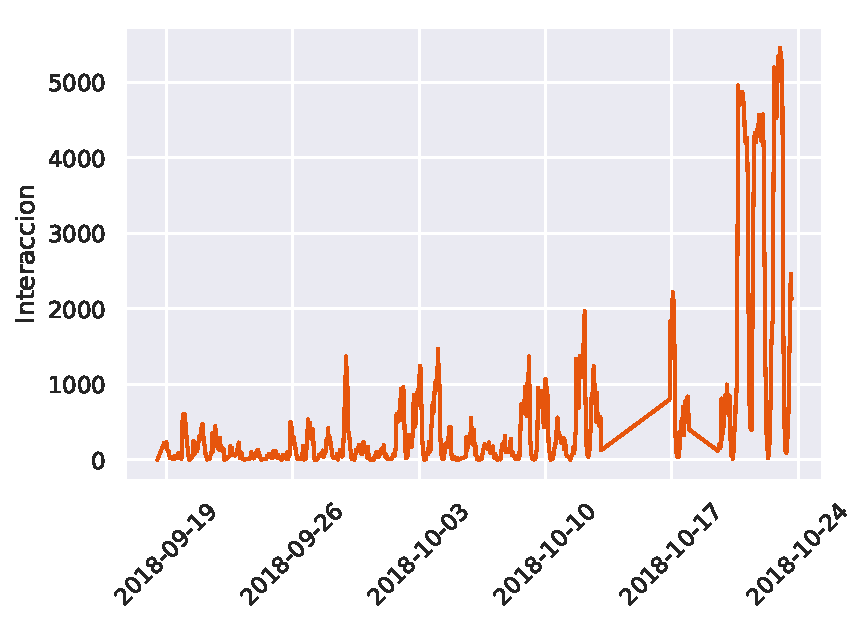
\includegraphics[width=0.75\textwidth]{Frequency_interactions.pdf}
\floatfoot{Insert note here.}
\end{figure}


\begin{figure}[h]
\caption{Tipo de interaccion por hora}
\centering
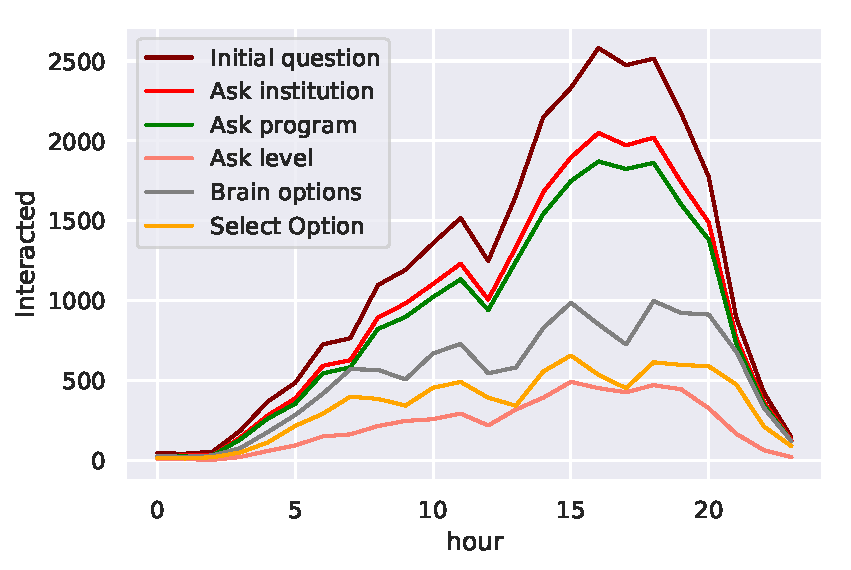
\includegraphics[width=0.75\textwidth]{Interaction_type.pdf}
\floatfoot{Insert note here.}
\end{figure}


\begin{figure}[h]
\caption{Discrepancia verdadero retorno salarial versus expectativa}
\centering
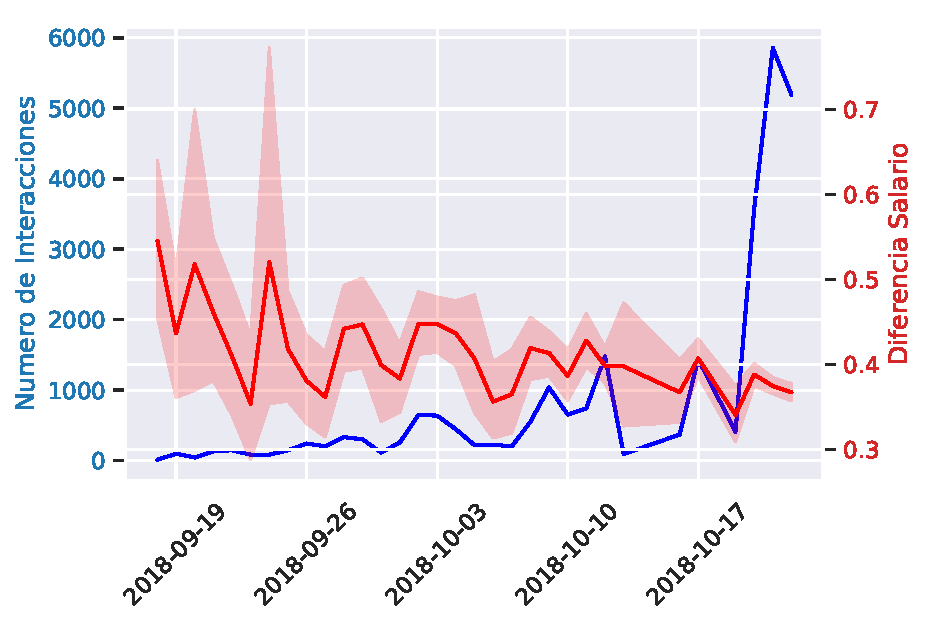
\includegraphics[width=0.75\textwidth]{Wage_deviation_byday.pdf}
\floatfoot{Insert note here.}
\end{figure}


\begin{figure}[h]
\caption{Descomposicion de discrepancia (tratado anteriormente vs tratado)}
\centering
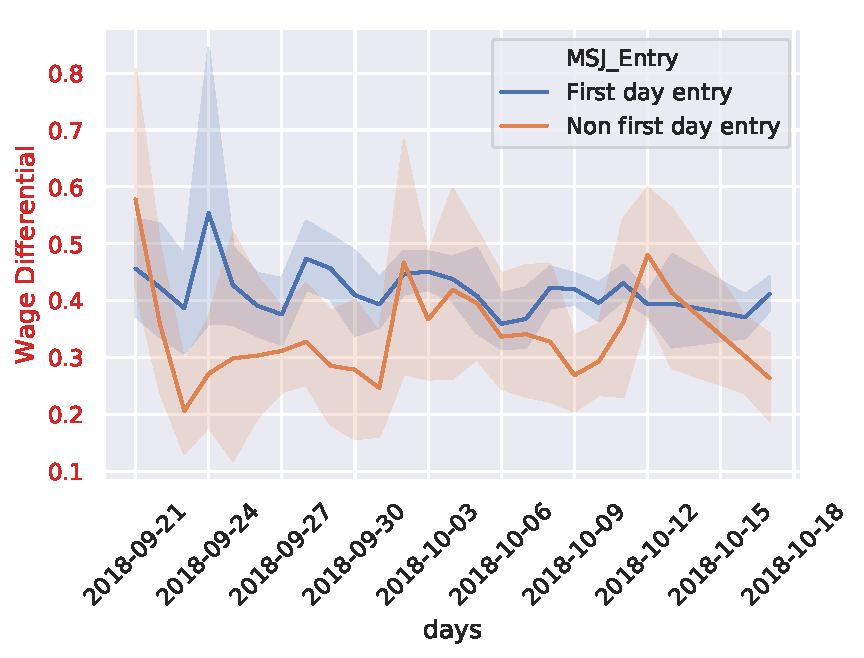
\includegraphics[width=0.75\textwidth]{Wage_deviation_by_entry.pdf}
\floatfoot{Insert note here.}
\end{figure}



\begin{figure}[h]
\caption{Desviacion por numero de interacciones}
\centering
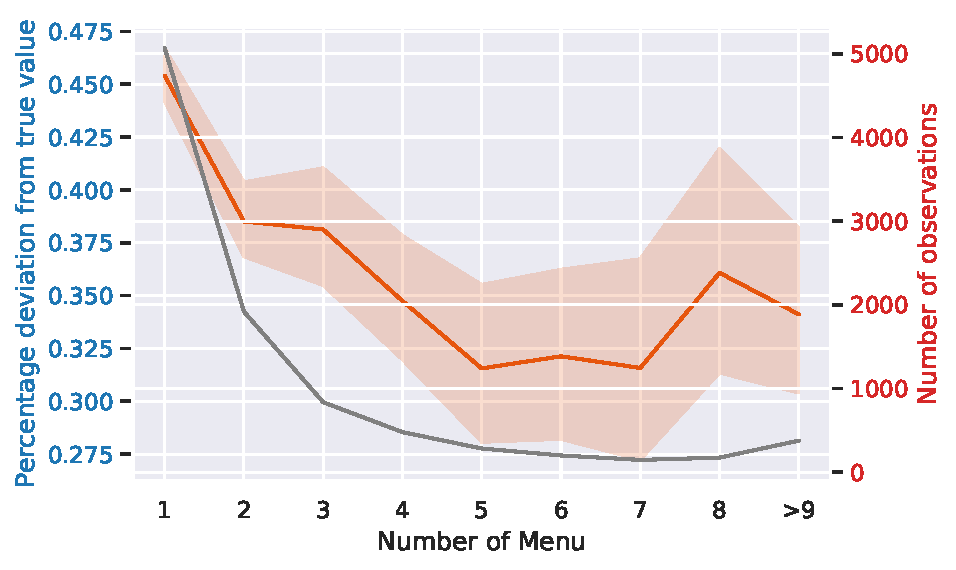
\includegraphics[width=0.75\textwidth]{Wage_deviation_by_nint.pdf}
\floatfoot{Insert note here.}
\end{figure}


\begin{figure}[h]
\caption{Descomposicion de la desviacion por numero de interacciones}
\centering
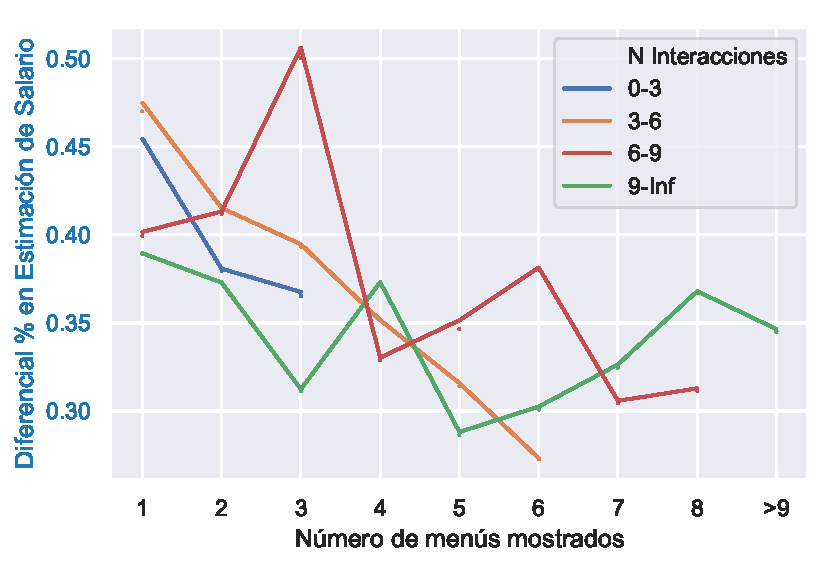
\includegraphics[width=0.75\textwidth]{Wage_deviation_decomposition.pdf}
\floatfoot{Insert note here.}
\end{figure}


\begin{figure}[h]
\caption{Take up del chatbot}
\centering
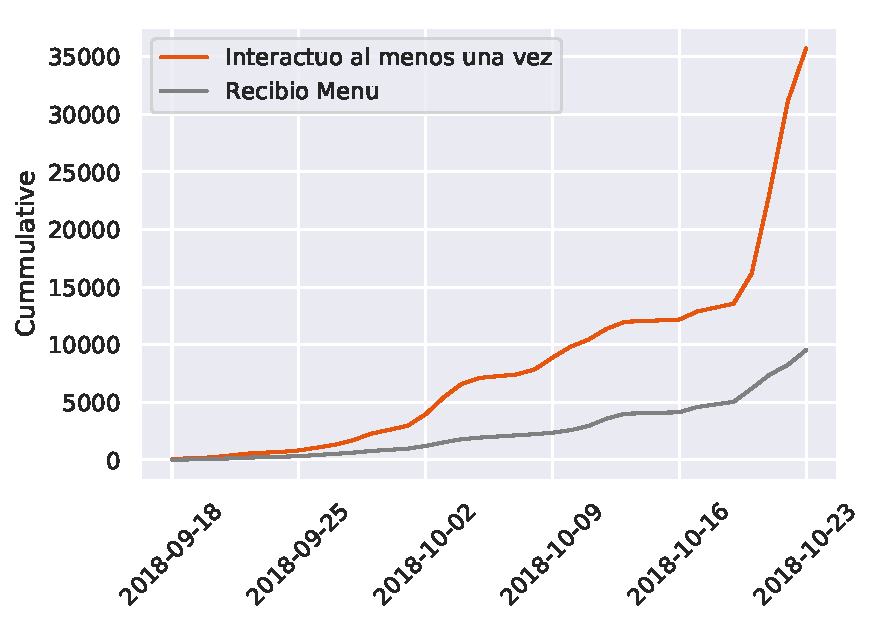
\includegraphics[width=0.75\textwidth]{Takeup_levels.pdf}
\floatfoot{Insert note here.}
\end{figure}


\begin{figure}[h]
\caption{Numero de estudiantes asignados a cada tratamiento}
\centering
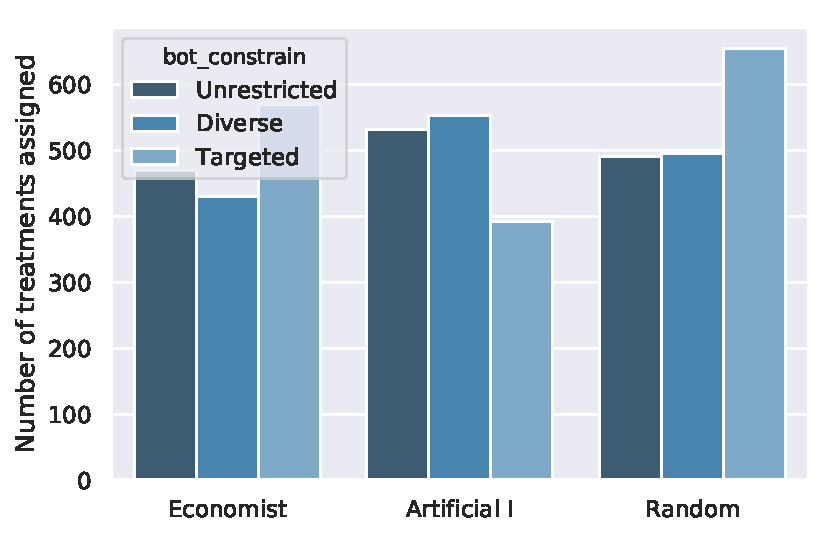
\includegraphics[width=0.75\textwidth]{Treatments_assigned.pdf}
\floatfoot{Insert note here.}
\end{figure}

\begin{figure}[h]
  \caption{Numero de clicks en outside option}
  \centering
  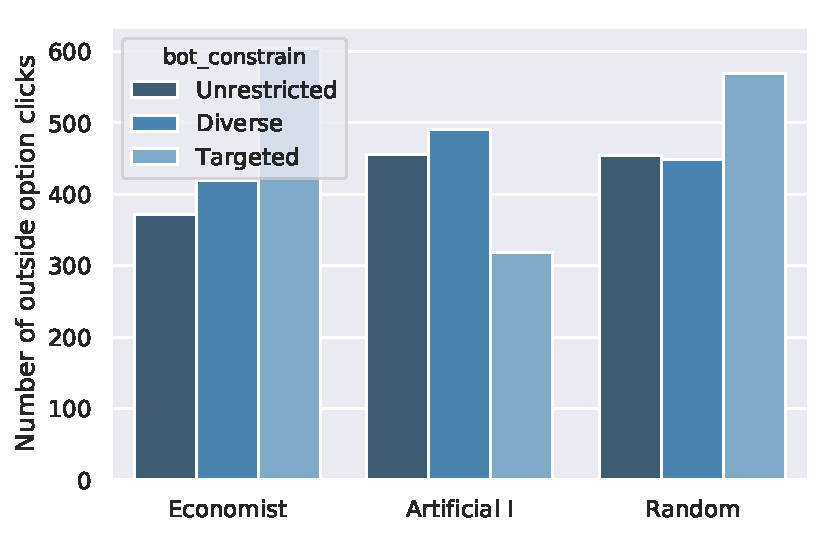
\includegraphics[width=0.75\textwidth]{Outside_option_clicks.pdf}
  \floatfoot{Insert note here.}
\end{figure}


\begin{figure}[h]
\caption{Porcentaje de clicks en outside option}
\centering
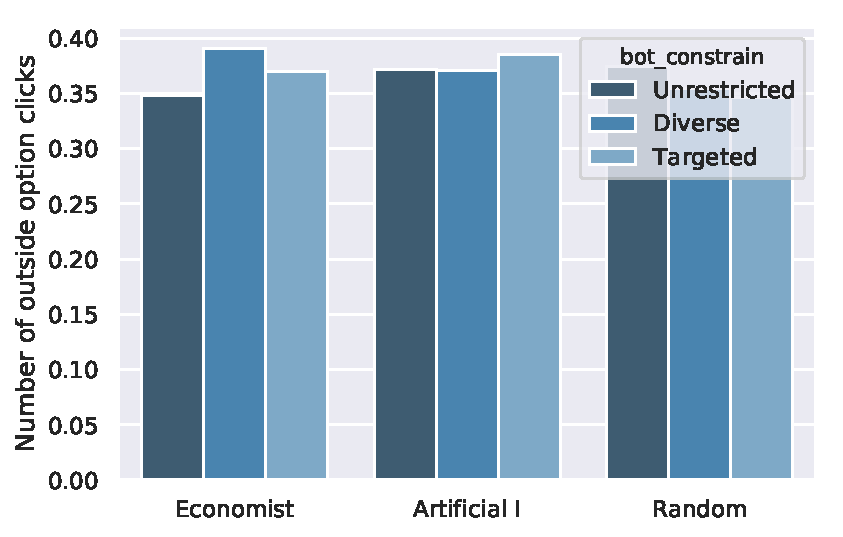
\includegraphics[width=0.75\textwidth]{outside_option_percentage.pdf}
\floatfoot{Insert note here.}
\end{figure}



\begin{figure}[h]
\caption{Numero de menus mostrados por tipo de tratamiento}
\centering
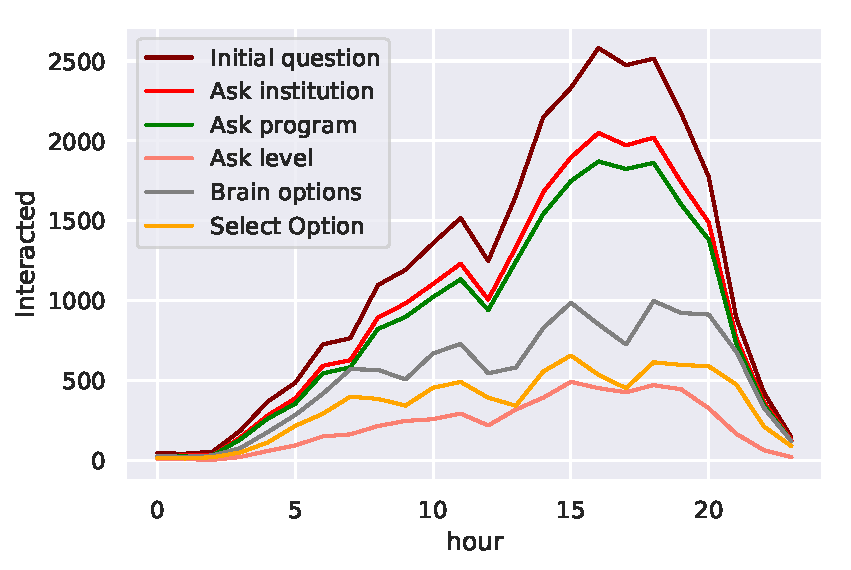
\includegraphics[width=0.75\textwidth]{Interaction_type.pdf}
\floatfoot{Insert note here.}
\end{figure}

\end{document}
